\documentclass[aspectratio=169]{beamer}
\usepackage[normalem]{ulem}


\usepackage{../theme/flagbot}
\usepackage{pgfpages}

%\setbeameroption{show notes on second screen}

\tikzstyle{freecell}=[fill=none]

\newcommand{\reg}[1]{\%\mintinline{asm}{#1}}
\newcommand{\hex}[1]{\mintinline{python}{0x#1}}
\newcommand{\naddr}[2]{\begin{tabular}{l}#1\\\hex{#2}\end{tabular}}
\newcommand{\docl}[1]{(\textbf{\href{#1}{Documentation}})}

\hypersetup{colorlinks,linkcolor=,urlcolor=brightblue}

\setbeamertemplate{navigation symbols}{}

\showsectionframe

%%%%%%%%%%%%%%%%%%%%%%%%%%%%%%%%%%%%%%%%%%%%%%%%%%%%%%%%%%%%%%%%%%%%%%%%%%%%%%%
% Title Setup
%%%%%%%%%%%%%%%%%%%%%%%%%%%%%%%%%%%%%%%%%%%%%%%%%%%%%%%%%%%%%%%%%%%%%%%%%%%%%%%
\title{Lesson 5: Constraint Solving and Symbolic Execution}
\subtitle{We'll have some fun}
\author{Luca Di Bartolomeo \and Leonardo Galli}
\date{\today}

\begin{document} 
\titleframe

\tocframe


{
\hidesectionframe
\showsubsectionframe
\section{Constraint Solving}
\subsection{General}

\begin{frame}[fragile]
    \frametitle{Problem: Annyoing Reverse Challenge}
    \begin{itemize}
        \item Already reversed good amount of challenge
        \item Now you know what conditions every byte of flag must fulfill
    \end{itemize}
    \begin{codebox}{c}
char vals[] = {0xe2, 0x37, 0xcf, 0xe4, 0xc2, 0x3a, 0x42, 0x6c, 0x6e, 0x92,
    0x5, 0x3a, 0xc5, 0xe6, 0xdf, 0x5c, 0x1f, 0x7, 0xe7, 0xd7, 0xd9, 0x1a,
    0xc7, 0xda, 0x63, 0x70, 0x7b, 0xf1, 0xf0, 0xf7, 0xf6, 0xf5};
int main(int argc, const char* argv[]) {
    char input[32];
    gets(input); // lets just imagine this removing newlines
    for (int i = 0; i < 32; i++) {
        char a = input[i] ^ (input[i] << 2);
        char b = (input[i] - i) ^ (input[i] + 20);
        if ((a ^ b) != vals[i]) return 1;
    }
    return 0;
}\end{codebox}
\end{frame}

% \begin{frame}
%     \frametitle{Solution: Constraint Solving}
%     {
%         \setbeamercolor{block title alerted} {fg = white, bg=brightgreen}
%         \setbeamercolor{block body alerted} {bg = darkgreen}
%     \begin{alertblock}{\textbf{Satisfiability modulo theories} (Boring Definition stolen from Wikipedia)}
%         An SMT instance is a formula in first-order logic, where some function and predicate symbols ahve additional interpretations, and SMT is the problem of determining whether such a formula is satisfiable
%         % A constraint satisfaction problem on finite domains (or CSP) is defined by a triplet $(\mathcal{X}, \mathcal{D}, \mathcal{C})$ where:
%         % \begin{itemize}
%         %     \item $\mathcal{X} = \{x_1, \dots, x_n\}$ is the set of variables of the problem;
%         %     \item $\mathcal{D} = \{\mathcal{D}_1, \dots, \mathcal{D}_n\}$ is the set of domains of the variables, i.e. $\forall k \in [n] \; x_k \in \mathcal{D}_k$
%         %     \item $\mathcal{C} = \{\mathcal{C}_1, \dots, \mathcal{C}_m\}$ is a set of constraints.
%         %         A constraint $\mathcal{C}_i = (\mathcal{X}_i, \mathcal{R}_i)$ is defined by a set $\mathcal{X}_i = \{x_{i_1}, \dots, x_{i_k}\}$ of variables and a relation $\mathcal{R}_i \subset \mathcal{D}_{i_1} \times \cdots \times \mathcal{D}_{i_k}$ which defines the set of values allowed simultaneously for the variables of $\mathcal{X}_i$.
%         % \end{itemize}
%     \end{alertblock}
%     }
% \end{frame}

\begin{frame}[fragile]
    \frametitle{Solution: Constraint Solving}
    \begin{enumerate}
        \item Define variables (usually input we control, in example \inlinecode[c]{char input[32]})
        \item Define domain of variables (usually printable characters)
        \item Define constraints, i.e. first-order logic formulas with equality (figured out by reversing)
        \item Use a tool (such as z3) to solve for your variables
    \end{enumerate}
\end{frame}

\begin{frame}
    \frametitle{Time Complexity}
    How long does a solver theoretically take?
    \pause
    \begin{alertblock}{\textbf{Running Time of Constraint Solvers}}
        It is very similar to the SAT problem. It comes to no surprise, that it is an NP-Complete Problem as well!
        Theoretically, it would take exponential time to solve!\\
        In practice, we have a small enough search space and independent parts.
        Additionally, specialized libraries have optimized code for solving these problems.
    \end{alertblock}
\end{frame}

\begin{frame}[fragile]
    \frametitle{z3 Installation}
    \begin{itemize}
        \item z3 does the heavy lifting of constraint solving for you
        \item usually you work with its python bindings, Z3Py
        \item installation should be easy via pip: \inlinecode[bash]{pip3 install z3-solver}
        \item \textbf{do not install z3!} 
    \end{itemize}

\end{frame}

\subsection{Defining Variables}

\begin{frame}[fragile]
    \frametitle{Considerations}
    \begin{itemize}
        \item similar to variables when programming, we need to specify the type
        \item usually, libraries support:
        \begin{itemize}
            \item integers
            \item real numbers
            \item even functions!
        \end{itemize}
        \item however, computers use neither integers or real numbers, but rather machine numbers
        \begin{itemize}
            \item often called \inlinecode[python]{BitVector}
            \item allows you to specify how many bits your machine number should have
        \end{itemize}
        \item usually, support for array types is either non existant or very limited
        \begin{itemize}
            \item this also applies to strings!
        \end{itemize}
    \end{itemize}
\end{frame}

\begin{frame}
    \frametitle{Working with Arrays and Strings}
    How can we define an array?
    \pause
    \begin{itemize}
        \item we define a sequence of variables
        \item since we will be scripting with python anyways, we can use arrays in python
    \end{itemize}
    Should we do the same for strings?
    \pause
    \begin{itemize}
        \item depends on the library, but usually yes (use python array of 8-bit BitVectors)
        \item for angr's implementation, it is usually more effective to define an $(8n)$-BitVector for a string of length $n$
    \end{itemize}
\end{frame}

\begin{frame}[fragile]
    \frametitle{Defining Variables with Z3Py}
    \begin{codebox}{python}
import z3

x = z3.Int('x') # all variables need a name
y = z3.Real('y')

flag = []
for i in range(32): # we know flag is at most 32 chars
    flag.append(z3.BitVec(f'flag_{i}', 8)) # char is 8 bits
    \end{codebox}
\end{frame}

\subsection{Defining the Domain}

\begin{frame}[fragile]
    \frametitle{Considerations}
    \begin{itemize}
        \item flag is always made out of printable characters:
        \begin{itemize}
            \item special characters: \inlinecode[python]{' !"#\$%&\'()*+,-./', 32 (0x20) - 47 (0x2f)}, \inlinecode[python]{':;<=>?@', 58 (0x3a) - 64 (0x40)}, \inlinecode[python]{'[\]^_`', 91 (0x5b) - 96 (0x60)}, \inlinecode[python]{'{|}~', 123 (0x7b) - 126 (0x7e)}
            \item digits: \inlinecode[python]{'0123456789', 48 (0x30) - 57 (0x39)}
            \item uppercase: \inlinecode[python]{'ABCDEFGHIJKLMNOPQRSTUVWXYZ', 65 (0x41) - 90 (0x5a)}
            \item lowercase: \inlinecode[python]{'abcdefghijklmnopqrstuvwxyz', 97 (0x61) - 122 (0x7a)}
        \end{itemize}
        \item try keeping your domain as small as possible!
        \item but, if exact length is unknown, some characters might be $0$!
        \item other types can be restricted like normal
        \begin{itemize}
            \item keep in mind - by default - numbers are signed!
            \item i.e. $x < 100$ allows $x = -200$
        \end{itemize}
    \end{itemize}
\end{frame}

\begin{frame}[fragile]
    \frametitle{Defining Domains with Z3Py}
    \begin{itemize}
        \item Z3Py has no real concept of domains, instead we just add constraints!
        \item for this, we need a \inlinecode[python]{Solver}
        \begin{itemize}
            \item stores constraints on variables
            \item will be used to solve these constraints
        \end{itemize}
        \item for now, we just add a few constraints
    \end{itemize}
\end{frame}

\begin{frame}[fragile]
    \frametitle{Defining Domains with Z3Py}
    \begin{codebox}{python}
s = z3.Solver() # create our solver

s.add(x < 100) # allows x = -200!
s.add(y < 100)
s.add(y > -100)

for c in flag:
    s.add(c >= ' ') # space is first printable character
    s.add(c <= '~') # tilde is last printable character\end{codebox}
\end{frame}

\subsection{Defining Constraints}

\begin{frame}[fragile]
    \frametitle{Considerations}
    \begin{itemize}
        \item when using BitVectors, there is no need for manual masking (e.g. \inlinecode[python]{x & 0xff}, ensuring only 8 bits used)
        \item usually, individual constraints are ANDed together
        \begin{itemize}
            \item if you need OR, create one constraint that is an OR of the individual constraints
        \end{itemize}
        \item keep your constraint count as low as possible, while also ensuring constraints are as ``tight"" as possible
        \begin{itemize}
            \item the less possible values your variables can take, the faster solving is
            \item for example, constrain flag to flag format, i.e. \inlinecode[python]{flag[:8] == 'flagbot'}
            \item the more constraints to fulfill, the slower solving is
        \end{itemize}
        \item when working with BitVectors, pay attention to signedness of operation
        \begin{itemize}
            \item by default, operations are signed
        \end{itemize}
    \end{itemize}
\end{frame}

\begin{frame}[fragile]
    \frametitle{Common Operations in Z3Py}
    \begin{itemize}
        \item arithmetic operations (unsigned counterparts): \inlinecode[python]{+, -, *, / (UDiv), % (URem)}
        \item bitwise operations: \inlinecode[python]{|, &, ^, ~}
        \item boolean operations: \inlinecode[python]{Or(a, b, ...), And(a, b, ...), Not(a), Xor(a, b), Implies(a, b)}
        \item comparison: \inlinecode[python]{<= (ULE), < (ULT), > (UGT), >= (UGE), ==}
        \item shifts: \inlinecode[python]{<<, >> (LShR), RotateLeft, RotateRight}
        \item concatenate multiple values (a will occupy bits starting at 0, b will follow after a, etc.): \inlinecode[python]{Concat(a, b, ...)}
        \item extract bits from BitVector: \inlinecode[python]{Extract(high, low, val)}
    \end{itemize}
    See \href{https://z3prover.github.io/api/html/namespacez3py.html}{Official Z3Py Documentation} for more!
\end{frame}

\begin{frame}[fragile]
    \frametitle{Defining Constrains in Z3Py}
\begin{codebox}{python}
for c in flag: # change our domain to allow 0
    s.add(z3.Or(c >= ord(' '), c == 0), c <= ord('~'))
# if one character is null, all following must be as well!
for i in range(len(flag)-1):
    s.add(z3.Implies(flag[i] == 0, flag[i+1] == 0))

z = z3.Int('z') # find prime smaller than 100
s.add(z3.ForAll([z], z3.Implies(z3.And(1 < z, z < x), x % z != 0)), 1 < x)
s.add(z3.ForAll([z], z3.Implies(z3.And(1 < z, z < y),
    z3.ToInt(y) % z != 0)), 1 < y)
vals = [0xe2, ..., 0xf5] # values extracted via reversing
for i, c in enumerate(flag): # add actual constraints
    a = c ^ (c << 2)
    b = (c - i) ^ (c + 20)
    s.add(a ^ b == vals[i])
\end{codebox}
\end{frame}

\subsection{Solving for Constraints}

\begin{frame}[fragile]
    \frametitle{Solving with Z3Py}
    Depends a lot on your library!
\begin{codebox}{python}
print(s.check()) # check() tries to find values satisfying all constraints
# prints 'sat' if values found, 'unsat' if not
print(s.model()) # model() gives you the actual values
# prints [flag_23 = 97,
# ...
# flag_19 = 102]
print("".join([chr(s.model().eval(c).as_long()) for c in flag]))
# prints 'flagbot{z3_makes_life_easy}\x00\x00\x00\x00\x00'
\end{codebox}

\end{frame}
}

\section{Angr}

\begin{frame}[fragile]
	\frametitle{Installation}
	\begin{itemize}
		\item \inlinecode[bash]{mkvirtualenv angr}
		\item \inlinecode[bash]{pip install angr}
	\end{itemize}
	\vspace{1em}
	OR
	\vspace{1em}
	\begin{itemize}
		\item \inlinecode[bash]{docker run -it angr/angr}
	\end{itemize}
\end{frame}

\begin{frame}[fragile]
	\frametitle{What are we talking about}
	\begin{itemize}
		\item \textbf{Claripy} - a data abstraction library
		\item \textbf{angr} - a concolic execution engine
	\end{itemize}
	\pause

	\vspace{3em}
	\emph{Around ~100k lines of python}
\end{frame}

\begin{frame}[fragile]
	\frametitle{Developers}
	\begin{center}
	
\includegraphics[scale=0.25]{shellphish.png}
	\end{center}

	\vspace{2em}
	\begin{center}
	UC Santa Barbara + Arizona State University
	\end{center}

	\pause
	\vspace{2em}

	For the DARPA Cyber Grand challenge
\end{frame}

\begin{frame}[fragile]
	\frametitle{What does concolic mean}
	{
		\Large
		\emph{
		``Concolic testing (a portmanteau of concrete and symbolic) is a hybrid
		software verification technique that performs \textbf{symbolic
		execution}, a classical technique that treats program variables as
		symbolic variables, along a \textbf{concrete execution} (testing on
		particular inputs) path''
		}
		\begin{flushright}
			\small
			Wikipedia
		\end{flushright}
	}
\end{frame}


\begin{frame}[fragile]
	\frametitle{What does concolic mean}
	\begin{center}
	\end{center}
	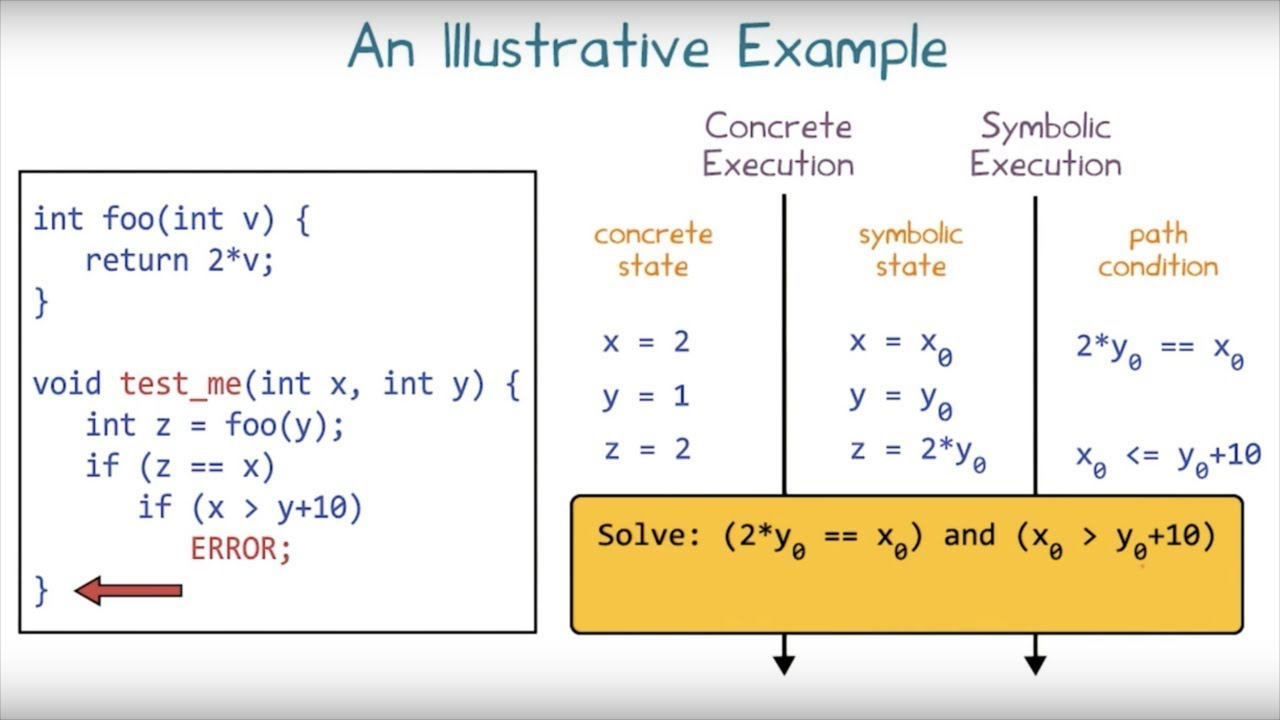
\includegraphics[scale=0.25]{symbolic.jpg}
\end{frame}


\begin{frame}[fragile]
	\frametitle{What does concolic mean}
	\begin{columns}
	\begin{column}{0.48\textwidth}
		\begin{center}
		\textbf{\Large Symbolic execution} \\
		\end{center}
		For each basic block, calculate all possible successors and all constraints necessary to get to a given successor

		\vspace{1em}

		Full control over the execution

		\vspace{1em}
		\vspace{1em}

		Quite slow

	\end{column}
	\begin{column}{0.48\textwidth}
		\begin{center}
		\textbf{\Large Concrete execution} \\
		\end{center}
		For each basic block, just execute it with your own damn CPU 

		\vspace{1em}
		\vspace{1em}

		Same execution control you would have with a debugger
		\vspace{1em}

		\emph{Many} orders of magnitude faster
	\end{column}
	\end{columns}
\end{frame}



\begin{frame}[fragile]
	\frametitle{Overview}
	\begin{center}
	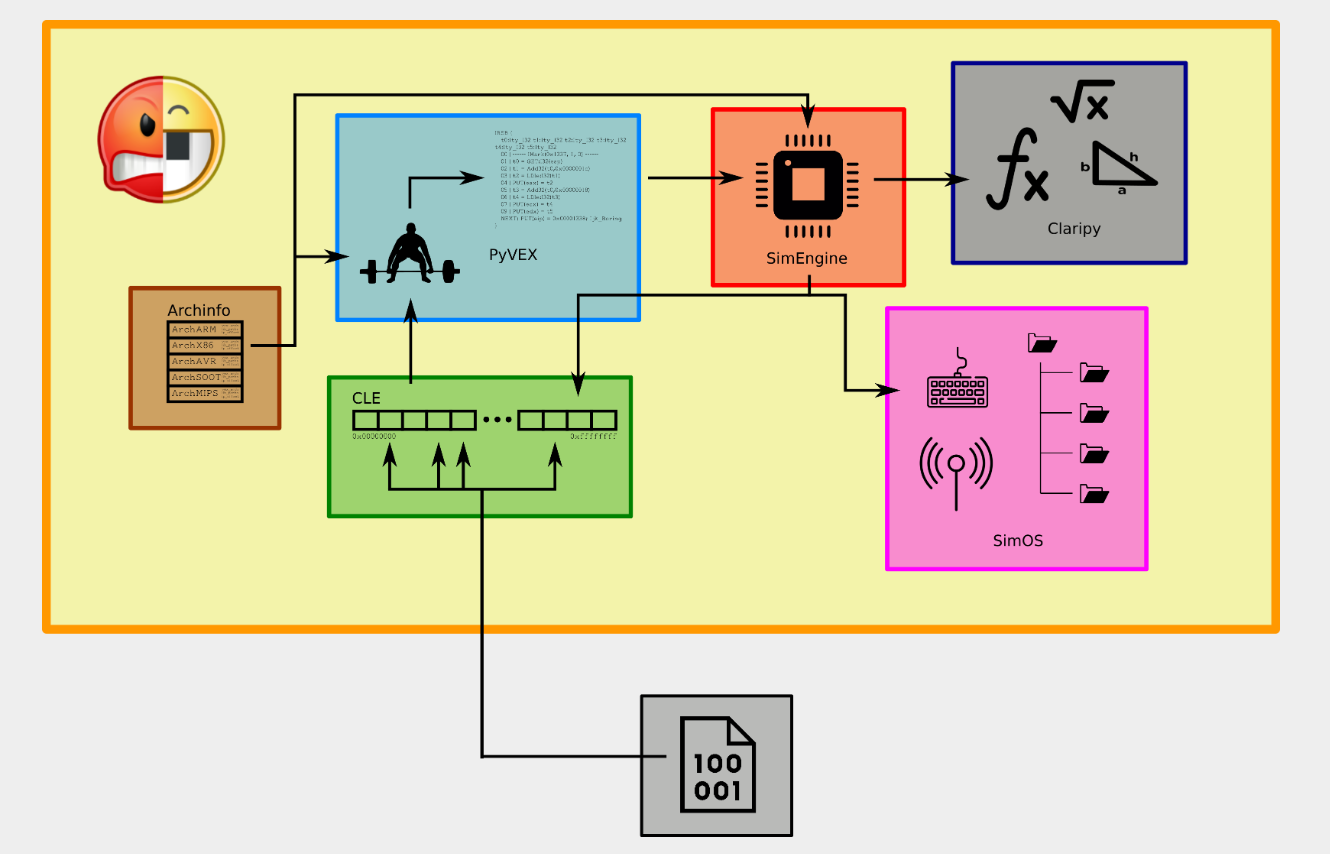
\includegraphics[scale=0.25]{angr_overview.png}
	\end{center}
\end{frame}


\begin{frame}[fragile]
	\frametitle{Actually, it's more like this}
	\begin{center}
		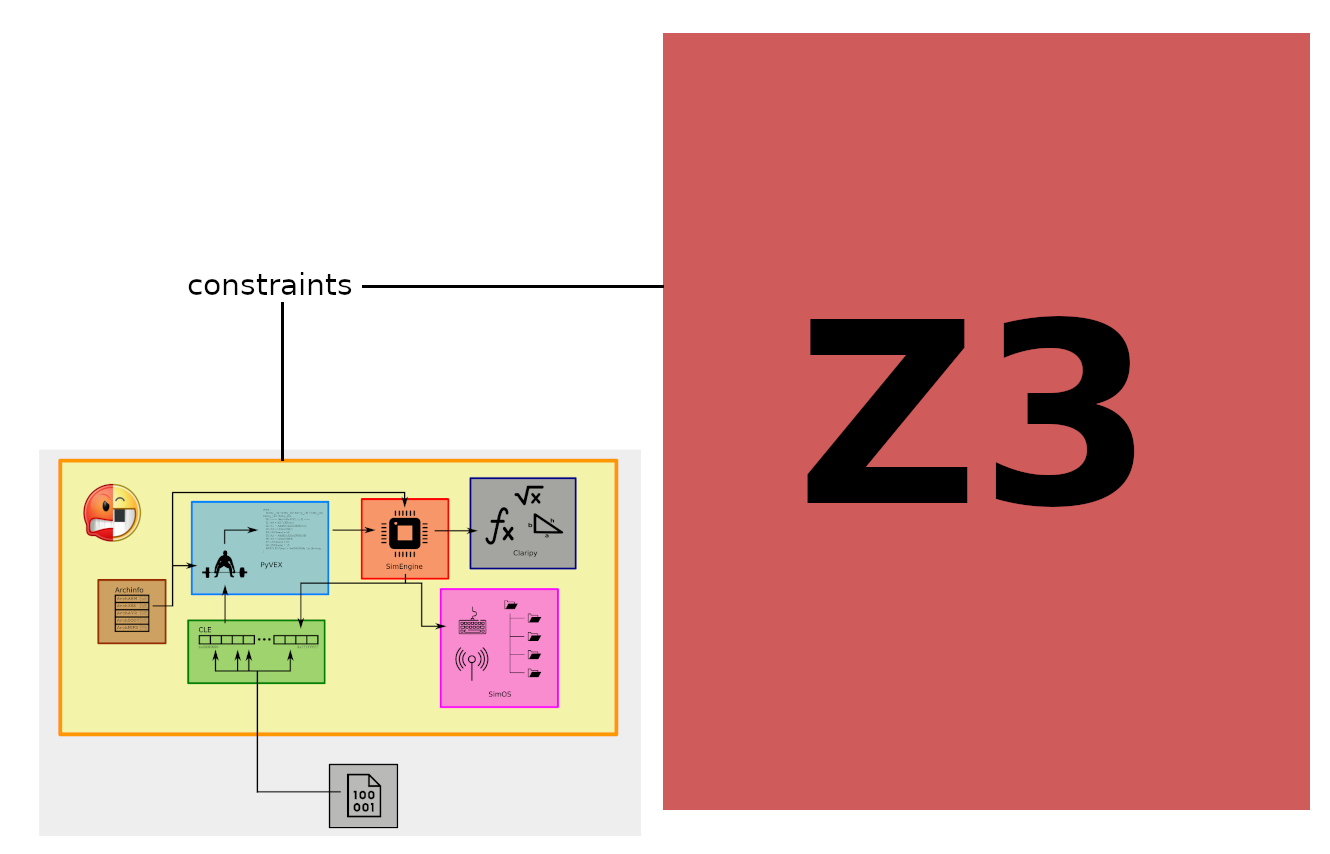
\includegraphics[scale=0.25]{true_overview.png}
	\end{center}
\end{frame}

\begin{frame}[fragile]
	\frametitle{Documentation}
	\texttt{Angr}'s documentation is like every cool recent state-of-the-art infosec tool
	\pause
	\vspace{1em}
	\begin{center}
		\Large
		\emph{it is basically non-existent}
	\end{center}
	\pause
    % IMO it's actually not *that* bad :P
	Your best bet is to have a look at what is \emph{pretending} to be the official
	documentation and a set of examples they provide on the angr website:
	\begin{itemize}
		\item \href{https://docs.angr.io/}{https://docs.angr.io/}
		\item \href{https://docs.angr.io/examples}{https://docs.angr.io/examples}
	\end{itemize}
	\pause
	And here again, you will find yourself having to look at the source code to understand how stuff works. Only this time it's Python, not C, so maybe it's a little better, I guess? Not sure though, honestly.
\end{frame}


\begin{frame}[fragile]
	\frametitle{Let's get our hands dirty}
	\begin{codebox}{python}
import angr
import claripy

project = angr.Project("./crackme") # load a binary

# This alone will take from 3 to 10 seconds
# If you think this is slow, oh boy, are you gonna change your mind\end{codebox}
\end{frame}


\begin{frame}[fragile]
	\frametitle{Let's get our hands dirty}
	\begin{codebox}{python}
import angr
import claripy

project = angr.Project("./crackme")
flag = claripy.BVS("flag", 8*100) # create a symbolic value

# first argument: name (does not really concern you)
# second argument: size in BITS (so here we have 100 chars)

# You can also use claripy.BVV() instead for a concrete (fixed) value \end{codebox}
\end{frame}


\begin{frame}[fragile]
	\frametitle{Let's get our hands dirty}
	\begin{codebox}{python}
import angr
import claripy

project = angr.Project("./crackme")
flag = claripy.BVS("flag", 8*50)
state = project.factory.full_init_state(stdin=flag)

# Here, we create an initial "state". There are many ways to do this:
# - full_init_state : quickly go over loading libs and go to main
# - entry_state     : bare-bones state corresponding to binary entry point
# - blank_state     : void state. Set starting address yourself.\end{codebox}
\end{frame}


\begin{frame}[fragile]
	\frametitle{Let's get our hands dirty}
	\begin{codebox}{python}
import angr
import claripy

project = angr.Project("./crackme")
flag = claripy.BVS("flag", 8*50)
state = project.factory.full_init_state(stdin=flag)
sm = project.factory.simulation_manager(state)
sm.explore(find=good_address, avoid=bad_address)

# Now, go and try to find desirable states!
# Arguments to 'find' and 'avoid' can be single addresses,
# lists of addresses or predicates on states

# A state can be in one of the following stashes:
# found - active - avoid - unsat - errored - deadended - unconstrained\end{codebox}
\end{frame}
% TODO: maybe explain the stashes?


\begin{frame}[fragile]
	\frametitle{Let's get our hands dirty}
	\begin{codebox}{python}
import angr
import claripy

project = angr.Project("./crackme")
flag = claripy.BVS("flag", 8*50)
state = project.factory.full_init_state(stdin=flag)
sm = project.factory.simulation_manager(state)
sm.explore(find=good_address, avoid=bad_address)
print (sm.found[0].solver.eval_upto(flag, 4, cast_to=bytes))

# Having found one (or more?) "good" states, we tell z3 to solve the
# constraints and give us up to 4 possible valid values for the 
# "flag" symbolic variable\end{codebox}
\end{frame}



\section{Demo}
\begin{frame}[fragile]
	\frametitle{Demo}
	\begin{center}
		Demo time!
	\end{center}
\end{frame}


\begin{frame}[fragile]
	\frametitle{Angr limitations}
	\begin{itemize}
		\item Path explosion
		\item Single-threaded
		\item It cannot cheat complex algos (e.g. crypto)
		\item You actually need to reverse part of the binary
	\end{itemize}
\end{frame}


\section{Tips and tricks}
\begin{frame}[fragile]
	\frametitle{Trick of the trade no. 1}
	\begin{center}
	{\Large Use \textsc{PyPy}!}
	\end{center}

	\begin{codebox}{bash}
pypy -m ensurepip
pypy -m pip install angr\end{codebox}
	\pause

	Depends on the case, but in my experience it gets you a 2x-8x speedup
\end{frame}


\begin{frame}[fragile]
	\frametitle{Trick of the trade no. 2}
	\begin{center}
	{\Large Give \textsc{Unicorn} a go!}
	\end{center}
	\begin{codebox}{python}
state = project.factory.blank_state(add_options=angr.options.unicorn)\end{codebox}
	\pause

	If you have to do a lot of concrete execution, this helps a lot
\end{frame}


\begin{frame}[fragile]
	\frametitle{Trick of the trade no. 3}
	\begin{center}
		{\Large You can load \textsc{Coredumps} in angr!}
	\end{center}
	\begin{codebox}{python}
proj = angr.Project("./coredump")\end{codebox}
\end{frame}


\begin{frame}[fragile]
	\frametitle{Trick of the trade no. 4}
	\begin{center}
		{\Large Symbolize \textsc{Arbitrary} memory!}
	\end{center}
	\begin{codebox}{python}
flag = claripy.BVS("flag", 8*8)
state.memory.store(flag, 0x800000)\end{codebox}
\end{frame}


\begin{frame}[fragile]
	\frametitle{Trick of the trade no. 5}
	\begin{center}
		{\Large Keep track of \textsc{Registers}!}
	\end{center}
	\begin{codebox}{python}
def lol(lsm):
	print(lsm.active[0].regs.rip)

sm.explore(find=address, avoid=address, step_func=lol)\end{codebox}
\end{frame}


\begin{frame}[fragile]
	\frametitle{Trick of the trade no. 6}
	\begin{center}
		{\Large Use symbolic \textsc{Arguments}!}
	\end{center}
	\begin{codebox}{python}
argv = [project.filename]
argv.append(sym_arg)
state = project.factory.entry_state(args=argv)\end{codebox}
\end{frame}


\begin{frame}[fragile]
	\frametitle{Trick of the trade no. 7}
	\begin{center}
		{\Large Impose your own \textsc{Constraints}!}
	\end{center}
	\begin{codebox}{python}
flag = claripy.BVS("flag", 8*100)
for byte in flag.chop(8):
        state.add_constraints(byte >= '\x20') # ' '
        state.add_constraints(byte <= '\x7e') # '~' \end{codebox}
\end{frame}


\begin{frame}[fragile]
	\frametitle{Trick of the trade no. 8}
	\begin{center}
		{\Large Implement stuff \textsc{Yourself}!}
	\end{center}
	\begin{codebox}{python}
class fixpid(angr.SimProcedure):
	def run(self):
		return 0x30

project.hook(0x4008cd, fixpid())\end{codebox}
\end{frame}



\begin{frame}[fragile]
	\frametitle{Trick of the trade no. 9}
	\begin{center}
		{\Large Tell angr's warnings to \textsc{Shut The Fuck Up}!}
	\end{center}
	\begin{codebox}{python}
state = project.factory.blank_state(
    add_options={angr.options.ZERO_FILL_UNCONSTRAINED_MEMORY,
                 angr.options.ZERO_FILL_UNCONSTRAINED_REGISTERS}))\end{codebox}
    \begin{itemize}
        \pause
        \item Actually useful in some cases, not just to make the output less annoying!
        \pause
        \item Usually, we can expect memory and registers to be zeroed initially. Being certain about it helps prevent path explosion
        (and generally makes things easier for angr)
        \pause
        % TODO: actually not sure if this is a valid point, since it will just (slowly) try to execute the native version then
        \item Some library functions that initialize memory to zero, such as \inlinecode[c]{explicit_bzero()},
            aren't recognized by angr {\tiny at the time of writing}
    \end{itemize}
\end{frame}

% TODO: reorder?
\begin{frame}[fragile]
    \frametitle{Trick of the trade no. 10}
    \begin{center}
        {\Large Be \textsc{Lazy}!}
    \end{center}
    \begin{codebox}{python}
state = ...
state.options |= {LAZY_SOLVES}
# you can also use the 'add_options' argument when creating the state\end{codebox}
% TODO: maybe use newer syntax for changing options??

\pause
\begin{itemize}
    \item By default, angr runs z3 to check states for \textbf{\color{brightgreen} satisfiability} at every simulation step.
    \begin{itemize}
        \item Might be good to avoid explosion by quickly throwing out impossible states
        \item but can be super slow
    \end{itemize}

\pause
    \item \inlinecode[python]{angr.sim_options.LAZY_SOLVES} \textbf{\color{brightpurple}defers} checking satisfiability \\ ``until absolutely necessary'' {\tiny [https://docs.angr.io/appendix/options]}
% TODO: cite properly?
    \begin{itemize}
        \item can speed up execution by 10x, maybe even more!
\pause
        % FIXME: this is kind of conjecture
        \item works well if a ``good'' path (along which to gather constraints) is easy to find and ``bad'' branches are easy to \inlinecode[python]{avoid}
        \item probably a bad idea if control flow is obfuscated (branches that are never taken, etc.)
    \end{itemize}
\end{itemize}

\end{frame}

\section{Troubleshooting}

\begin{frame}[fragile]
    \frametitle{Dealing with Symbolic Strings}

    \label{slide:symbolic_strings}

    \begin{itemize}
        \item angr's \texttt{SimProcedure}s of string functions such as \inlinecode[c]{strlen} assume symbolic strings to be \textbf{\color{brightpurple}at most 60 bytes long} by default
        \item If a string needs to be longer than that, {\footnotesize or you specifically constrain it to be longer than 60,} you get an \textbf{\color{orange}unsatisfiable} state :(
\pause
        \item Easy fix: \begin{codebox}{python}
buf_size = 128
flag = claripy.BVS("flag", 8*buf_size)

state = ...
state.libc.buf_symbolic_bytes   = buf_size
state.libc.max_str_len          = buf_size
# might want to use max() instead
# to make sure you're not making anything smaller\end{codebox}

    \end{itemize}

\end{frame}


\begin{frame}[fragile]
    \frametitle{Unsatisfiable States}

    \begin{itemize}
        \item A state becomes unsatisfiable when its constraints \textbf{\color{brightpurple}contradict} each other
        \begin{itemize}
            \item informally: ``this cannot possibly happen on a machine''
\pause
            \item constraints may be path constraints derived from control flow, or ones you manually added
            \begin{codebox}{c}
void foo(int x) {
    if (x == 42) {
        puts("forty-two");
        if (x == 43) {
            // states here are always unsat
            // (unless you manually mess with them)
            puts("this is fine");
            puts("absolutely no bitflips from cosmic radiation");
            system("sudo rm -rf /");
        }
    }
}\end{codebox}
        \end{itemize}
    \end{itemize}
\end{frame}


\begin{frame}[fragile]
    \frametitle{Debugging Unsatisfiable States}

    \begin{itemize}
        \item You can access a state's constraints (e.g. in a Python debugger) using \inlinecode[python]{state.solver.constraints}
\pause
        \begin{itemize}
            \item but that may be a lot of constraints, so which ones are actually wrong?
        \end{itemize}
\pause
        \item \inlinecode[python]{unsat_core()} gives you a \textbf{\color{brightpurple}subset of contradicting constraints}
        % XXX: it actually gives you a list, I think, but that's beside the point
        \begin{itemize}
            \item actually how I found out about the issue with symbolic string lengths from slide \ref{slide:symbolic_strings}
\pause
            \item need to enable an option to use:\begin{codebox}{python}
state = ...
state.options |= {angr.sim_options.CONSTRAINT_TRACKING_IN_SOLVER}
# you can also use 'add_options'

sm = project.factory.simulation_manager(state)
sm.explore(...)

# assume you have an unsat state that *should* be satisfiable
print("one of these is false: ", sm.unsat[0].solver.unsat_core())
\end{codebox}% TODO: actually test printing, but I don't see why it shouldn't work
        \end{itemize}
    \end{itemize}
\end{frame}
%\begin{frame}[fragile]
    %\frametitle{Frequently Asked Questions}
	%Q: Why is it called radare2? Where is radare1?
	%\begin{itemize}
		%\item I don't know. I don't think anyone does.
    %\end{itemize}

	%Q: I found out that I have installed a very recent verion, \textit{\textless insert any number here\textgreater}.\\
	%Is it okay if I use it?
	%\begin{itemize}
		%\item No. Use the git one.
	%\end{itemize}
	%Q: I will never remember all those cryptic commands and options. I don't think radare2 is for me.
	%\begin{itemize}
		%\item This is not a question.
	%\end{itemize}
	
	%Q: Honestly, this FAQ sucks, do you have anything better?
	%\begin{itemize}
		%\item You can forward all your complaints to \texttt{gallile@student.ethz.ch}
	%\end{itemize}
%\end{frame}

\section{Other tools}

\begin{frame}[fragile]
    \frametitle{Other tools}
	\begin{itemize}
		\item Triton
		\item KLEE
		\item S2E
	\end{itemize}
	\vspace{3em}
	%\hline
	\pause
	\vspace{1em}
	\begin{itemize}
		\item Less suitable for a quick hack
		\item More stable; more documented
		\item Actually used by many companies $\rightarrow$ will probably be supported for a long time
	\end{itemize}

	Exception: Manticore
\end{frame}

\section{Challenge}

\begin{frame}[fragile]
    \frametitle{Challenge}
    {
        \begin{alertblock}{\textbf{Angry bomb}}
			This one's easy - it's the famous reversing bomb, 6 stages (or more?)
			of pure fun disarming. But wait, it's with a twist! Now you actually 
			need to solve each phase with angr. No manual reversing allowed! \\
            \textbf{Hints:} Whenever you feel really angry -- scream, it will help. Source: am Italian\\
            \textbf{Files:} \href{https://cdn.vis.ethz.ch/ctf/chals/bomb.zip}{bomb.zip}\\
            \textbf{Author:} CMU Labs
        \end{alertblock}
    }
\end{frame}
\end{document}
